%!TEX root = ../report_template.tex
\section{Results and Discussion}
The introduced students-per-teacher ratio aggregates the number of children per teacher, either for each federal state or school type. This section will compare it to the Abitur grades, repeaters, and budgets. Due to the data representation, the Abitur grades can only be analyzed for the German average. Nevertheless, the repeaters and budgets are analyzed for each federal state.

One of the key findings of this analysis is the strong correlation between the average grades across all federal states and the students-per-teacher ratio in German grammar schools. As shown in \autoref{fig:regression-stt-grade}, the relationship between both is nearly linear and contains neither clusters nor outliers. Thus, a smaller students-per-teacher ratio strongly correlates to better Abitur grades, with a Pearson correlation coefficient of $r=0.98$.

\begin{figure}[ht]
    \centering
    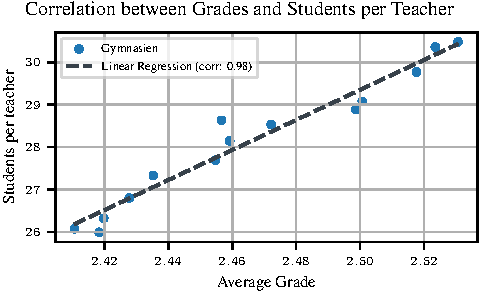
\includegraphics{fig/fig_correlation_grades_students_per_teacher.pdf}
    \caption{Linear regression on the students-per-teacher ratio by average Abitur grade. The resulting regression line (\textcolor{TUred}{\rule[-0.2ex]{0.5em}{2pt} \rule[-0.2ex]{0.5em}{2pt}}) is calculated over the aggregated average overall grammar schools (\textcolor{TUlightblue}{\tikz\draw[fill={TUlightblue}] (0,0) circle (0.25em);}) in Germany.}
    \label{fig:regression-stt-grade}
\end{figure}

This confirms the initial hypothesis of the high influence of the students-per-teacher ratio on grades and is consistent with the findings of prior research \cite{kasau_onesmus_mulei_pupil-teacher_2016,koc_impact_2015,dickson_economic_1984}.

However, the Abitur grades only give an insight into grammar schools. So additionally, the correlations with repeaters and budgets are shown in \autoref{fig:heatmap_correlation_students_per_teacher_repeaters_budget}. Note, that the Pearson correlation coefficients for each state are normalized to the used color map scale.

\begin{figure}[ht]
    \centering
    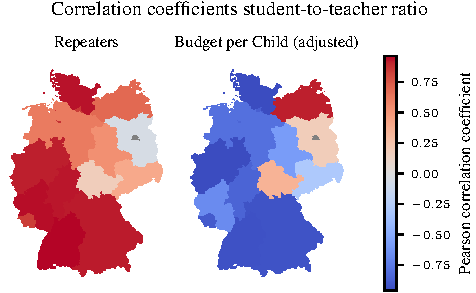
\includegraphics{fig/fig_heatmap_correlation_students_per_teacher_repeaters_budget.pdf}
    \caption{Pearson correlation coefficients between the students-per-teacher ratio and the relative repeater count (left) and the inflation-adjusted average budget per child (right). Missing values are shown in \textcolor{TUdark}{dark gray}.}
    \label{fig:heatmap_correlation_students_per_teacher_repeaters_budget}
\end{figure}

The findings presented in \autoref{fig:heatmap_correlation_students_per_teacher_repeaters_budget} support a  positive correlation between the students-per-teacher ratio and the number of repeaters in most federal states. In contrast, the right heatmap (\autoref{fig:heatmap_correlation_students_per_teacher_repeaters_budget}) indicates a negative correlation between the students-per-teacher ratio  and budget per child for the same states. Furthermore, there is a big difference between \emph{old} and \emph{new} federal states for both correlations. Especially, the results for Thüringen and Brandenburg diverge from the average in both maps. Rather, Mecklenburg-Vorpommern differs most in the budget per child from the other states.

However,  an increase in the number of students in the new federal states can explain the different correlations in the budget per child\footref{footnote:teachers-children}. Since the per-child budget has increased in all states\footref{footnote:budget}, the schools got more money in total. This results in more vacancies at schools \cite{kultusminister_konferenz_lehrkrafteeinstellungsbedarf_2023} and other investments, like digitalization and maintenance of schools \cite{bundesministerium_fur_bildung_und_forschung_fortschrittsbericht_2022}. But in the short term, there will be more teachers needed as available \cite{kultusminister_konferenz_lehrkrafteeinstellungsbedarf_2023}. As \autoref{fig:teacher_contracts} indicates, this leads to a high variance in the distribution of teacher contract types, especially for the new federal states. This results in a higher students-per-teacher ratio with the same budget.

In contrast, the anomaly for the repeaters involves more aspects of the educational system, like the different curricula or conditions for repeating a class. The conditions for repetitions vary between federal states and are just an indicator rather than a measure of educational quality \cite{klemm_klassenwiederholungen_2009}. Hence, a complete explanation for these results involves more datasets and effects. Although, the majority of federal states have a positive correlation with the number of repeaters, it indicates that a small students-per-teacher ratio is beneficial for challenged students.

Moreover, the other states indicate that a higher budget per child results in a smaller students-per-teacher ratio. Hence, the number of repeaters decreases with the students-per-teacher ratio.